\chapter{Расчет экономической эффективности системы}
\section{Введение}
Для оценки экономической эффективности программно-аппаратного продукта требуется:
\begin{itemize}
\item определить целесообразность разработки;
\item определить трудоёмкость и затраты на создание;
\item определить показатели экономической эффективности разработки.
\end{itemize}

Результатом выполнения данной части является обоснование технической, экономической и научной значимости и целесообразности продукта в соответствии с~\cite{EconomicsMethodic}. Объектом технико-экономического анализа является программная система мониторинга состояния ЛА на основе методов интеллектуального анализа данных.

\section{Определение целесообразности разработки}
Для обоснования целесообразности разработки продукта необходимо:
\begin{itemize}
\item выбрать аналог (если таковой имеется);
\item сформулировать перечень функциональных характеристик по предлагаемому варианту разработки продукта;
\item определить конкретные уровни характеристик и их значимость;
\item определить индекс технического уровня программного продукта.
\end{itemize}

Функционально-технические характеристики разрабатываемого программного продукта представлены в таблице~\ref{tab:economics:characteristics}.

\begin{table}[h]
\caption{Функционально-технические характеристики}
\nohyphenation
\label{tab:economics:characteristics}

\begin{tabular}{|C{120.05pt}|C{77.95pt}|C{72pt}|C{72pt}|C{108pt}|}
\hline
\multirow{2}{\hsize}{\centering{Функциональные характеристики}} & \multirow{2}{\hsize}{\centering{Единица измерения}} & \multicolumn{2}{C{144pt}|}{Величина функциональных характеристик} & \multirow{2}{\hsize}{\centering{Значимость характеристик}} \\
\cline{3-4}
 & & Аналог & Новый вариант & \\
\hline
Простота использования & По 10-бальной шкале & 2 & 9 & 0.05 \\
\hline
Быстродействие & По 10-бальной шкале & 5 & 10 & 0.2 \\
\hline
Открытость & По 10-бальной шкале & 3 & 10 & 0.15 \\
\hline
Точность вычислений & По 10-бальной шкале & 8 & 8 & 0.2 \\
\hline
Надёжность & По 10-бальной шкале & 9 & 7 & 0.2 \\
\hline
\end{tabular}
\end{table}

Индекс технического уровня разрабатываемого программного продукта определяется по формуле~\ref{eq:economics:techindex}:

\begin{equation}\label{eq:economics:techindex}
J_{\text{\sl ТУ}} = \sum\limits_{i=1}^{n} \frac{\alpha_i}{\alpha_{i0}} \mu_i ,
\end{equation}

\begin{description}
\item[где $\alpha_i$]~---~уровень $i$-й функционально-технической харатеристики проектируемого алгоритма;
\item [$\alpha_{i0}$]~---~уровень $i$-й функционально-технической харатеристики базового алгоритма;
\item [$\mu_i$]~---~значимость $i$-го параметра;
\item [$n$]~---~количество рассматриваемых параметров.
\end{description}

\begin{equation*}
J_{\text{\sl ТУ}} = \frac{9}{2} \cdot 0.05 + \frac{10}{5} \cdot 0.2 + \frac{10}{3} \cdot 0.15 + \frac{8}{8} \cdot 0.2 + \frac{7}{9} \cdot 0.2 = 1.48.
\end{equation*}

Значение показателя технического уровня разрабатываемого программного продукта превышает 1 и равно 1.48. Полученный результат является подтверждением целесообразности разработки продукта.

\section{Определение трудоемкости и затрат на создание ПП}
Основой для определения затрат на создание ПП является показатель трудоемкости работ. В таблице~\ref{tab:economics:costsstructure} представлена структура затрат труда на создание ПП.

\begin{table}[h]
\caption{Структура затрат труда на создание ПП}
\label{tab:economics:costsstructure}
\nohyphenation

\begin{tabular}{|C{31pt}|C{320pt}|C{112pt}|}
\hline
№ п/п & Наименование (стадии) этапа работ & Доля работ на стадии (этапе) в общем объёме работ, \% \\
\hline
1 & Анализ предметной области и изучение средств разработки & 3 \\
\hline
2 & Изучение программируемой задачи & 5 \\
\hline
3 & Определение входных и выходных данных & 3 \\
\hline
4 & Анализ методов решения задачи & 5 \\
\hline
5 & Составление структуры ПП & 4 \\
\hline
6 & Технико-экономическое обоснование выбора вариантов решения задачи & 5 \\
\hline
7 & Уточнение и доработка выбранного варианта решения & 3 \\
\hline
8 & Создание ПП & 35 \\
\hline
9 & Отладка ПП & 22 \\
\hline
10 & Испытание и анализ работы ПП в реальных условиях & 10 \\
\hline
11 & Составление технической документации & 5 \\
\hline
 & ИТОГО & 100 \\
\hline
\end{tabular}
\end{table}

Затраты труда определяются по формуле~\ref{eq:economics:workcosts}.

\begin{equation}\label{eq:economics:workcosts}
t_{\text{\sl ПРТ}} = t_{\text{\sl О}} + t_{\text{\sl И}} + t_{\text{\sl А}} + t_{\text{\sl К}} + t_{\text{\sl ОТ}} + t_{\text{\sl Д}}
\end{equation}

\begin{description}
	\item[$B = 2$] --- увеличение затрат труда на изучение и постановку задачи вследствие их сложности и новизны;
	\item[$K = 0.8$] --- коэффициент квалификации разработчика;
	\item[$Q = q \cdot K_c \cdot (1 + \sum_{}^{n} K_k) = 500 \cdot 1.5 \cdot (1 + (0.2 + 0.1)) = 975.$]
	\item[$t_{\text{\sl О}} = 40$] --- затраты труда на подготовку описания задачи;
	\item[$t_{\text{\sl И}} = \frac{Q \cdot B}{75 \cdot K} = 32.5$] --- затраты труда на изучение и постановку задачи;
	\item[$t_{\text{\sl А}} = \frac{Q}{20 \cdot K} = 60.94$] --- затраты труда на проектирование системы;
	\item[$t_{\text{\sl К}} = \frac{Q}{10 \cdot K} = 121.88$] --- затраты труда на программирование;
	\item[$t_{\text{\sl ОТ}} = \frac{Q}{5 \cdot K} = 243.75$] --- затраты труда на отладку программы;
	\item[$t_{\text{\sl Д}} = \frac{1.75 \cdot Q}{15 \cdot K} = 142.19$] --- затраты труда на подготовку документации.
\end{description}

Таким образом, $t_{\text{\sl ПРТ}} = 40 + 32.5 + 60.94 + 121.88 + 243.75 + 142.19 = 641.26$.

\section{Определение исполнителей}
Исполнители указаны в таблице~\ref{tab:economics:stuff}.

\begin{table}[h]
\caption{Исполнители}
\label{tab:economics:stuff}
\nohyphenation

\begin{tabular}{|C{99.25pt}|C{120.5pt}|C{113.4pt}|C{120.45pt}|}
\hline
Категория исполнителей & Число исполнителей & Зарплата с учетом премии (руб./мес.) & Часовые тарифные ставки, руб. \\
\hline
Инженер-программист & 1 & 60000 & 360 \\
\hline
\end{tabular}
\end{table}

\section{Расчет заработной платы исполнителей}
Оплата труда персонала определяется на основе общей трудоёмкости создания ПП по формуле~\ref{eq:economics:salary}.

\begin{equation}\label{eq:economics:salary}
\text{\sl ЗП}_\text{\sl ПП} = \sum_{i=1}^{k} \text{\sl Т}_i \cdot \overline{\tau_i} \text{,}
\end{equation}

\begin{description}
	\item[где $k$] --- количество этапов;
	\item[$\text{\sl Т}_i$] --- трудоёмкость $i$-го этапа;
	\item[$\overline{\tau_i}$] --- средняя дневная тарифная ставка оплаты $i$-го этапа.
\end{description}

Результаты приведены в таблице~\ref{tab:economics:salary}.

\begin{table}[H]
\caption{Заработная плата исполнителей}
\label{tab:economics:salary}
\nohyphenation

\begin{tabular}{|C{36.7pt}|C{192.2pt}|C{96.25pt}|C{59.65pt}|C{81.15pt}|}
\hline
№ п/п & Наименование этапов и работ & Трудоёмкость стадии (чел.-ч.) & Часовая ставка (руб/ч) & Зарплата за работу (руб) \\
\hline
1 & Анализ предметной области и изучение средств разработки & 40 & 360 & 6000 \\
\hline
2 & Изучение программируемой задачи & \multirow{3}{\hsize}{\centering{32.5}} & \multirow{3}{\hsize}{\centering{360}} & \multirow{3}{\hsize}{\centering{11700}} \\
\cline{1-2}
3 & Определение входных и выходных данных & & & \\
\cline{1-2}
4 & Анализ методов решения задачи & & & \\
\hline
5 & Составление структуры ПП & \multirow{3}{\hsize}{\centering{60.94}} & \multirow{3}{\hsize}{\centering{360}} & \multirow{3}{\hsize}{\centering{21938.40}} \\
\cline{1-2}
6 & Технико-экономическое обоснование выбора вариантов решения задачи & & & \\
\cline{1-2}
7 & Уточнение и доработка выбранного варианта решения & & & \\
\hline
8 & Создание ПП & 121.88 & 360 & 43876.80 \\
\hline
9 & Отладка ПП & \multirow{2}{\hsize}{\centering{243.75}} & \multirow{2}{\hsize}{\centering{360}} & \multirow{2}{\hsize}{\centering{87750}} \\
\cline{1-2}
10 & Испытание и анализ работы ПП в реальных условиях & & & \\
\hline
11 & Составление технической документации & 142.19 & 360 & 51188.40 \\
\hline
 & ИТОГО & 641.26 & -- & 230853.60 \\
\hline
\end{tabular}
\end{table}

\section{Социальные отчисления}
Социальные отчисления основных исполнителей составляет 30.2\% от $\text{\sl ЗП}_\text{\sl ПП}$.

$\text{\sl З}_\text{СО} = 230853.60 \cdot 0.302 = 69717.79$ (руб.)

\section{Накладные расходы}
Под накладными расходами понимаются расходы на электроэнергию в период первого полугодия эксплуатации системы. Они расчитываются по формуле~\ref{eq:economics:overheadcosts}.

\begin{equation}\label{eq:economics:overheadcosts}
K_\text{\sl ЭЭ} = N_\text{\sl раб.дн.} \cdot \sum P \cdot N_\text{\sl часов} \cdot N_\text{\sl лет} \cdot C_\text{\sl ЭЭ} \text{,}
\end{equation}

\begin{description}
	\item[где $N_\text{\sl раб.дн.}$] --- количество рабочих дней в году;
	\item[$\sum P$] --- суммарная потребляемая в час мощность оборудования (компьютер используется в течение всего рабочего дня, а принтеры~–-- в среднем в течение половины рабочего дня);
	\item[$N_\text{\sl часов}$] --- количество рабочих часов в день;
	\item[$N_\text{\sl лет}$] --- количество лет разработки или использования системы;
	\item[$C_\text{\sl ЭЭ}$] --- стоимость одного киловатт/часа электроэнергии.
\end{description}\smallskip

Таким образом, $K_\text{\sl ЭЭ} = 224 \cdot 4.3 \cdot 8 \cdot 0.5 \cdot 4.5 = 17337.6$ (руб.)

\section{Прочие расходы}
Прочие прямые расходы –-- это расходы на использование машинного времени. Система будет разрабатываться в течение 90 дней в среднем по 8 часов ежедневно. При стоимости машинного времени 13 руб./час, получаем:

$\text{\sl З}_\text{М.В.} = 90 \cdot 8 \cdot 13 = 9360.00$ (руб.)

Сведём все расходы на создание и эксплуатацию системы в таблицу~\ref{tab:economics:totalcost}.

\begin{table}[h]
\caption{Сводная таблица расходов}
\label{tab:economics:totalcost}
\nohyphenation

\begin{tabular}{|C{35.45pt}|C{177.2pt}|C{92.15pt}|C{106.3pt}|}
\hline
№ п/п & Виды расходов & Расходы, руб. & Удельный вес, \% \\
\hline
1 & Заработная плата разработчиков & 230853.60 & 70.54 \\
\hline
2 & Социальные отчисления & 69717.79 & 21.3 \\
\hline
3 & Накладные расходы & 17337.6 & 5.3 \\
\hline
4 & Прочие расходы & 9360 & 2.86 \\
\hline
 & ИТОГО & 327268.99 & 100 \\
\hline
\end{tabular}
\end{table}

\section{Расчет стоимости}
Цена программного продукта определяется исходя из принципа обеспечения безубыточности деятельности организации, получения прибыли, позволяющей выплатить обязательные платежи в бюджет и инвертировать расширение деятельности.

Цена первоначальной продажи определяется по формуле~\ref{eq:economics:firstsale}.

\begin{equation}\label{eq:economics:firstsale}
\text{\sl Ц}_{\text{\sl НТПр}}^{n} = \text{\sl З}_\text{\sl НТПр} + \frac{\text{\sl ЗП}_\text{\sl ПП} \cdot \rho_\text{\sl ЗП}}{100} \text{,}
\end{equation}

\begin{description}
	\item[где $\text{\sl З}_\text{\sl НТПр}$] --- текущие затраты на создание, определяющиеся по формуле~\ref{eq:economics:currentcosts}:
	\begin{equation}\label{eq:economics:currentcosts}
	\text{\sl З}_\text{\sl НТПр} = \text{\sl ЗП}_\text{\sl пп} + \text{\sl З}_\text{\sl М.В.} \text{;}
	\end{equation}
	\item[$\text{\sl ЗП}_\text{\sl ПП}$] --- оплата труда основного персонала в общих текущих затратах на создание программного продукта;
	\item[$\rho_\text{\sl ЗП}$] --- уровень рентабельности (прибыли по отношению к оплате труда персонала), обеспечивающий безубыточность деятельности ($\rho_\text{\sl ЗП} = 200\%$).
\end{description}

Таким образом,

$\text{\sl З}_\text{\sl НТПр} = 230853.60 + 9360 = 240213.60 \text{ руб.};$

$\text{\sl Ц}_{\text{\sl НТПр}}^{n} = 240213.60 + \frac{230853.60 \cdot 200}{100} = 701920.80 \text{ руб.}$

\section{Оценка экономической эффективности}
Так как данная дипломная работа связана с разработкой алгоритмов и программ, то $\text{\sl Э}_\text{\sl НТП}$ определяется по формуле~\ref{eq:economics:economy}.

\begin{equation}\label{eq:economics:economy}
\text{\sl Э}_\text{\sl НТП} = \sum_{i=1}^{n} \varDelta T_\text{\sl мi} \cdot C_{BT} \text{,}
\end{equation}

\begin{description}
	\item[где $\varDelta T_\text{\sl мi}$] --- экономия машинного времени, ч.;
	\item[$C_{BT}$] --- стоимость одного машинного часа, руб.;
	\item[$n = 3000$] --- количество задач, решаемых в год.
\end{description}
\smallskip

$\text{\sl Э}_\text{\sl НТП} = 3000 \cdot 8 \cdot 50 = 1 200 000$ (руб.)
\smallskip

Уровень экономической эффективности ($\text{\sl Е}_\text{\sl ПП}$) и срок окупаемости затрат на создание алгоритмов и ПП ($T_{OK}$) определяется по формулам~\ref{eq:economics:efficiency}~и~\ref{eq:economics:paybacktime}.

\begin{equation}\label{eq:economics:efficiency}
\text{\sl Е}_\text{\sl ПП} = \frac{\text{\sl Э}_\text{\sl НТП}}{\text{\sl Ц}_{\text{\sl НТПр}}}
\end{equation}
\begin{equation}\label{eq:economics:paybacktime}
T_{OK} = \frac{1}{\text{\sl Е}_{\text{\sl ПП}}}
\end{equation}

Таким образом,

$\text{\sl Е}_\text{\sl ПП} = \frac{1 200 000}{701920.80} = 1.71;$

$T_{OK} = \frac{1}{1.71} = 0.59$ (года).\smallskip

Так как уровень экономической эффективности составляет 1.71, то можно сделать вывод о том, что разработанный ПП выгоден с экономической точки зрения.

\section{Календарное планирование}
Календарный план работ представлен в таблице~\ref{tab:economics:calendarplan}.

\begin{longtable}{|C{16pt}|C{130pt}|C{64pt}|C{80pt}|C{78pt}|C{80pt}|}
\caption{Календарный план работ}
\label{tab:economics:calendarplan}
\\ \hline
№ п/п & Наименование этапов (стадий, видов работ) & Удельный вес, \% & Трудоемкость этапа, чел.-ч. & Кол-во исполнителей & Длительность этапа \\ \hline
\endfirsthead
\LTcontcaption{tab:economics:calendarplan}
\\ \hline
№ п/п & Наименование этапов (стадий, видов работ) & Удельный вес, \% & Трудоемкость этапа, чел.-ч. & Кол-во исполнителей & Длительность этапа \\ \hline
\endhead
1 & Анализ предметной области и изучение средств разработки & 6.24 & 40 & 1 & 6 \\
\hline
2 & Изучение программируемой задачи & 2.31 & 14.8 & 1 & 1 \\
\hline
3 & Определение входных и выходных данных & 1.21 & 7.76 & 1 & 5 \\
\hline
4 & Анализ методов решения задачи & 1.55 & 9.94 & 1 & 14 \\
\hline
5 & Составление структуры ПП & 3.7 & 23.74 & 1 & 6 \\
\hline
6 & Технико-экономическое обоснование выбора вариантов решения задачи & 4 & 25.66 & 1 & 6 \\
\hline
7 & Уточнение и доработка выбранного варианта решения & 1.8 & 11.54 & 1 & 4 \\
\hline
8 & Составление ПП & 19.01 & 121.88 & 1 & 39 \\
\hline
9 & Отладка ПП & 22 & 141.08 & 1 & 16 \\
\hline
10 & Испытание и анализ работы ПП в реальных условиях & 16.01 & 102.67 & 1 & 13 \\
\hline
11 & Составление технической документации & 22.17 & 142.19 & 1 & 8 \\
\hline
 & ИТОГО & 100 & 641.26 & 1 & 118 \\
\hline
\end{longtable}

Производственный цикл каждого этапа определяется по формуле~\ref{eq:economics:cycle}.

\begin{equation}\label{eq:economics:cycle}
T_\text{\sl ц j} = \frac{T_j}{t_\text{\sl рд} \cdot q_j} \text{,}
\end{equation}

\begin{description}
	\item[где $T_j$] --- трудоёмкость $j$-ой стадии ($j$-го этапа), чел.-час.;
	\item[$t_\text{\sl рд}$] --- продолжительность рабочего дня, час.;
	\item[$q_j$] --- количество работников, одновременно участвующих в выполнении работ на $j$-ой стадии ($j$-м этапе), чел.
\end{description}

На основании данных таблицы ~\ref{tab:economics:calendarplan} построен сетевой график (рисунок~\ref{fig:economics:schedule}).

\begin{figure}[h]
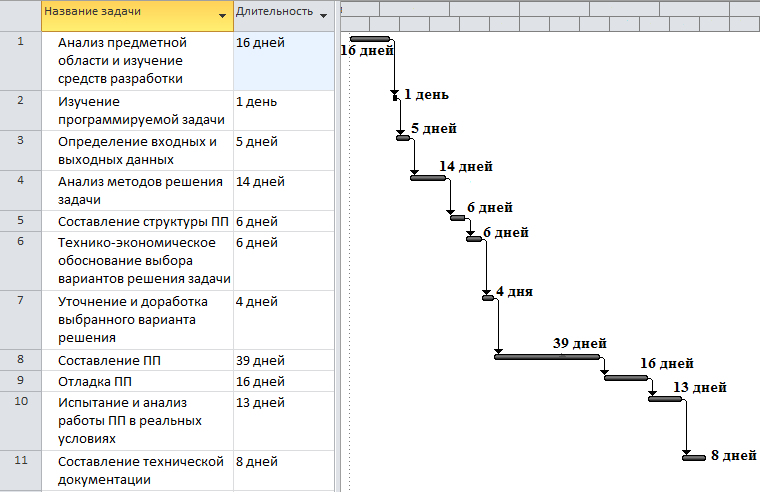
\includegraphics[width=0.9\textwidth, keepaspectratio]{int_op_schedule}
\caption{Календарный план-график работ}\label{fig:economics:schedule}
\end{figure}

\section{Выводы}
В экономической части дипломной работы получены следующие значения экономических показателей:

\begin{itemize}
	\item Технический уровень $J_{\text{\sl ТУ}} = 1.48$. Значение этого показателя должно быть больше 1. Полученное значение говорит о высоком техническом уровне разрабатываемого изделия.
	\item Уровень экономической эффективности $\text{\sl Е}_\text{\sl ПП} = 1.71$.
\end{itemize}

На основании показателей экономической эффективности считаем разрабатываемую систему экономически эффективной и внедрение в производство целесообразным.